\documentclass[10pt,a4paper]{article}
\usepackage[utf8]{inputenc}
\usepackage{amsmath}
\usepackage{amsfonts}
\usepackage{amssymb}
\usepackage{makeidx}
\usepackage{titling}
\usepackage{blindtext}
\usepackage{graphicx}
\usepackage{caption}
\usepackage{subfig}
\usepackage{wrapfig}
\setlength{\intextsep}{0pt}
\usepackage[export]{adjustbox}
\usepackage[a4paper,margin=1in]{geometry}
\author{Erik Rosvall, Viktor Karlsson, Lucas Grönlund \& Marcus Alsterman}
\title{Machine Learning Advanced course \\ String Subsequence Kernel}



%\setcounter{chapter}{1}
\begin{document}
	\begin{titlingpage}
		\maketitle
		\begin{abstract}
			Trying to solve text classification creates many issues, mainly feature extraction and handling multi labeled data that might be unbalanced. This report looks at how a String Subsequence Kernel can solve the mentioned problems in conjunction with a SVM. This report goes through how Lodhi et al has presented and validated their algorithm with both recursive and approximate implementations. Lastly we present our own incremental improvement of the approximate String Subsequence Kernel by the use of additional halt conditions within the recursion. 
		\end{abstract}
	\end{titlingpage}
	
	\section{Introduction}
	
In the area of machine learning, classification of unseen data is of great interest. For this to be possible feature vectors of the input data are needed which is trivial for some types of data, but not so for text documents. Transforming the data into a \textit{feature space} by quantifying some aspect of the document, and then compare similarity between data points through their inner product is called the \textit{kernel method}. Using the '\textit{kernel trick}' for the \textit{support vector machine} (SVM) classifier the explicit transform into this feature space can be avoided.% which in many cases is what enables the method to be used since the feature spaces can be of very high dimensionality, in some cases even infinite.

The paper \cite{lodhi} presents a new method of performing feature extraction from text documents which Lohdi et al. names \textit{string subsequence kernel} (SSK). The SSK is compared with two other feature extraction methods, namely \textit{word kernel} (WK) and \textit{n-gram kernel} (NGK). Kernels are not the only successful type of method in the text classification field, neural networks as well as a \textit{fastText} \cite{joulin2016bag} have shown great results. These are regarded as state of the art algorithms and will compared to the kernels methods presented above. 

Throughout \cite{lodhi} the dataset used for classification was the \textit{Reuters-21578 dataset} consisting of news articles from Reuters news agency. \textit{Modified Apte}, also known as ModeApte, was used to split this data set into 7769 training documents and 3019 test documents, divided into 90 classes. These classes are however not mutually exclusive which is common for text data, a document can for example be tagged with both 'earn' and 'acquisition' which is an extension making the classification more involved.

The aim of this report is to replicate the results in \cite{lodhi} regarding the SSK, where the emphasis is put on the approximative implementation. We have therefore used Python packages such as \texttt{Sklearn} and \texttt{Numpy} for supplying SVM algorithms and other conveniences, but written code for all three kernels ourselves. Further, we have put no effort into replicating the results regarding the combination of kernels Lohdi et al. presents since it did not improve the classification performance in any significant way. Finally, we also propose a possible computational complexity reduction of the SSK since this is the the major downside with the algorithm.


	
	\section{Method}
	
\subsection{Support Vector Machine}
The SVM is a binary classifier separating two classes of data with a maximum margin decision boundary. Since this is not of central interest in this article or \cite{lodhi}, we suppose the details of this algorithm to be known. The algorithm can be formulated in a way such that the training features only occur in inner products with other training feature vectors, which often is called the \textit{dual formulation}. When the problem is formulated in this way the kernel trick can be used, which lets us avoid having to explicitly transform our input data into the kernel space. 

Since the Reuters dataset have text documents assigned to multiple classes, a problem often called\textit{ multi-label-} or \textit{vector output classification}, the SVM cannot be used directly since it is a binary classifier. To deal with this issue we implemented a \textit{one-vs-rest} approach. Thus, we train one classifier for each class with data from that class regarded as positive samples and the rest of the dataset as negative samples. This algorithm was imported from the \texttt{sklean} package in python. 

\subsection{String subsequence kernel}
\cite{lodhi} proposes a feature extraction method for text documents, extending the n-gram approach to features also being non-contiguous substrings. The feature vectors for each document is thus created through first generating all such subsequences, from all documents in the dataset, of length $ k $. Each such substring is regarded as a dimension of the feature space. 

The transformation of a document to this feature space is then performed "simply" trough finding all occurrences of these subsequences and weighing them according to how compactly the sequence is embedded in the text. This is handled through the introduction of a \textit{decay factor} $ \lambda \in (0,1) $, which lets us put smaller emphasis on less compactly embedded subsequences than ones more compactly embedded in the document. An example of this, presented in \cite{lodhi}, is if we consider the subsequence \textbf{c-a-r} which is more compactly found in the document '\textbf{car}d' than in   '\textbf{c}ust\textbf{ar}d', giving the former a value of $ \lambda^3 $ and the latter $ \lambda^6 $, where the exponent directly corresponds to the length of the sequence for which the subsequence is contained.

To not introduce unnecessary confusion we will present the definition of a SSK exactly as the definition presented in \cite{lodhi}. 

\subsubsection{Definition - String subsequence kernel}
Let $ \Sigma $ be a finite alphabet. A string is a finite seqence of characters from $ \Sigma $, including the empty sequence. For strings $s,t$ we denote by $|s|$ the length of the string $ s = s_1 \dots s_{|s|} $, and by $ st $ the string obtained by concatenating the strings $ s $ and $ t $. The string $ s[i:j] $ is the substring $ s_i, \dots s_j $ of $ s $. We say that $ u $ us a subsequence of $ s $, if there exist indices $ \boldsymbol{i} = (i_1, \dots, i_{|u|}) $, with $ 1 \leq i_1 < \dots < i_{|u|} \leq |s| $, such that $ u_j = s_{i_{j}}$, for $ j = 1, \dots, |u|, $ or $ u = s[\boldsymbol{i}] $ for short. The length $ l(\boldsymbol{i}) $ of the subsequence in $ s $ is $ i_{|u|} - i_1 +1 $. We denote by $ \Sigma^n $ the set of all finite strings of length $ n $, and by $ \Sigma^* $ the set of all strings 
\begin{equation}\label{eq:all_Strings}
\Sigma^* = \bigcup^{\infty}_{n=0}\Sigma^n
\end{equation}
We now define the feature spaces $ F_n = \mathbb{R}^{\Sigma^{n}} $. The feature mapping $ \phi $ for a string $ s $ is given by defining the $ u $ coordinate $ \phi_u(s) $ for each $u \in \Sigma^n  $ We define 
\begin{equation}
\phi_u(s) = \sum_{\boldsymbol{i}:u=s[\boldsymbol{i}]} \lambda^{l(\boldsymbol{i})}
\end{equation}
for some $ \lambda \in (0,1) $. These features measure the number of occurrences of subsequences in the string $ s $ weighting them according to their lenghts. Hence, the inner product of the feature vectors for two strings $ s $ and $ t $ give a sum over all common subsequences weighted according to their frequency of occurrence and lengths
\begin{align*}\label{key}
K_n(s,t) &= \sum_{u\in\Sigma^n} \langle \phi_u(s) \cdot \phi_u(t) \rangle = \sum_{u \in \Sigma^n} \sum_{\boldsymbol{i}:u=s[\boldsymbol{i}]} \lambda^{l(\boldsymbol{i})} \sum_{\boldsymbol{j}:u=t[\boldsymbol{j}]} \lambda^{l(\boldsymbol{j})} \\
& =  \sum_{u \in \Sigma^n} \sum_{\boldsymbol{i}:u=s[\boldsymbol{i}]}  \sum_{\boldsymbol{j}:u=t[\boldsymbol{j}]} \lambda^{l(\boldsymbol{i}) + l(\boldsymbol{j})}
\end{align*}


To prove our understanding of this definition we construct a unique example, which also illustrates how the feature vectors look. Consider two documents containing the words \textit{fail} or \textit{sail}. 

\begin{table}[h]
	\centering
\begin{tabular}{|c|c|c|c|c|c|c|c|c|c|c|c|c|c|}
	\hline 
	& f-a & f-i & f-l & a-i & a-l & i-l & s-a & s-i & s-l & a-t & l-i & l-t & i-t \\ 
	\hline 
	$\phi(fail)$ & $ \lambda^2 $ & $ \lambda^3 $ &$ \lambda^4 $  &  $ \lambda^2 $& $ \lambda^3 $  & $ \lambda^2 $ & 0 & 0 & 0 & 0 & 0 & 0 & 0 \\ 
	\hline 
	%$\phi(alit)$ & 0 & 0 & 0 & $\lambda^3$ & $\lambda^2$ & 0 & 0 & 0 & 0 & $\lambda^4$ & $\lambda^2$ & $\lambda^3$ & $\lambda^2$ \\ 
	%\hline 
	$\phi(sail)$ & 0 & 0 & 0 & $\lambda^2$ & $\lambda^3$ & $\lambda^2$ & $\lambda^2$ & $\lambda^3$ & $\lambda^4$ & 0 & 0 & 0 & 0 \\ 
	\hline 
\end{tabular} 
\caption{Feature vectors for two simple documents.}
\end{table}

To calculate the similarity between the documents \textit{fail} and \textit{sail} we simply calculate the inner product between their respective feature vectors, resulting in the kernel value $ K_2(fail,sail)  = 2\lambda^4 + \lambda^6 $, where the subindex represent the subsequence length $ n $. An other example which we later used to prove that our implementation of the SSK was correct was the kernel values \cite{lodhi} presents for the documents \textit{'science is organized knowledge'} and \textit{'wisdom is organized life'}. These were: $ K_1 = 0.580 $, $ K_2 = 0.580$, $ K_3 = 0.478, K_4=0.439, K_5 = 0.406, K_6 = 0.370 $.

To explicitly calculate all the features for documents present in the Reuters dataset would require impractical amounts of computations, which is why \cite{lodhi} presents a recursive formulation for the kernel values. We will again present these as they were in the paper, since we followed them exactly in our implementation. 

\subsubsection{Definition - Recursive computation of the subsequence kernel}
\begin{align*}
	K'_{0}(s,t) & = 1, for\ all\ s,t \\
	K'_i(s,t) & = 0, if\ \min(|s|,|t|) < i \\
	K_i(s,t) & = 0, if\ \min(|s|,|t|) < i \\
	K'_i(sx,t) & = \lambda K'_i(s,t) + \sum_{j:t_j=x} K'_{i-1}(s,t[1:j-1])\lambda^{|t|-j+2}, \hspace{15pt} i = 1, \dots n-1 \\	
	K_{n}(sx,t) & = K_n(s,t) + \sum_{j:t_j = x}K'_n-1(s,t[1:j-1])\lambda^2
\end{align*}  
This recursive formulation leaves the computational complexity at $ \mathcal{O}(n|s||t|^2]) $ which can be improved using the efficient computation \cite{lodhi} presents, through first evaluating
\begin{equation*}\label{key}
K''_i(sx,t) = \sum_{j:t_j = x}K'_{i-1}(s,t[1:j-1])\lambda^{|t|-j+2}.
\end{equation*}
Observing that $ K'_i(s,t) $ can be evaluated with the recursion:
\begin{equation*}\label{key}
K'_i(sx,t) = \lambda K'_i(s,t) + K''_i(sx,t)
\end{equation*}
one can then observe that $ K''_i(sx,tu) = \lambda^{|u|}K''_i(sx,t)$, in the case that $ x $ does not occur in $ u $, and otherwise 
\begin{equation*}\label{key}
K''_i(sx,tx) = \lambda \left( K''_i(sx,t) + \lambda K'_{i-1}(s,t) \right).
\end{equation*} 
With this implementation the computational complexity reduces to $ \mathcal{O}(n|s||t|) $.



\subsubsection{Approximating string subsequence kernel}
To test SSK on the entire Reuters dataset an approximative approach is needed, we call this aSSK. This is enabled through the general empirical kernel map presented in \cite{Scholkopf} which states that if we have a set $ S = \{s_i\} $ of vectors such that these vectors, when transformed into the kernel space, are both orthogonal and span the entire kernel space (that is $ \mathcal{K}(s_i,s_j) = C\delta_{ij} $), we can write the kernel value for any other two feature vectors
\begin{equation}\label{eq:kernel_approx}
\mathcal{K}(x,z) = \dfrac{1}{C}\sum_{s_i \in S}\mathcal{K}(x,s_i)\mathcal{K}(z,s_i)
\end{equation}

If we instead of constructing a set $ S $ with full cardinality limit ourselves to only choosing a subset $ \tilde{S} \subset S $ we can approximate the true kernel value with fewer computations. How 'close' this approximation $ \mathcal{K} $ is to the true kernel matrix $ K $ can be measured through the alignment of the two matrices, defined as

\begin{equation}\label{key}
A(K,\mathcal{K}) = \dfrac{\langle K, \mathcal{K}\rangle_{F}}{\sqrt{\langle \mathcal{K}, \mathcal{K}\rangle_{F} \langle K, K\rangle_{F} }}
\end{equation}
Here the subindex F indicates that the inner product is Frobenius normed defined as $ \langle K_1,K_2 \rangle_{F} = \sum_{i}\sum_{j}K_1(x_i,x_j)K_2(x_i,x_j) $.

To generate $ \tilde{S} $ we followed \cite{lodhi}, first choosing the substring length $ n $, then counting all contiguous substrings of length $ n $ in all the documents and finally constructed $ \tilde{S} $ with the x most occurring substrings. Using the alignment measure between the approximated kernel matrix and the exact one, we studied the the effect the number of features had on the approximation. 
. 
\subsection{N-gram kernel}
The n-gram kernel (NGK) transforms text documents to the feature space trough  considering contiguous subsequences of length $ n $, called \textit{n-grams}. The value of each dimension in the feature space of a document is thus the number of occurrences of that n-gram in the document. 

With this approach all information encoded in the word order in the document is lost. The method has nonetheless proven useful, as we will see later.

\subsection{Word kernel}
The word kernel (WK) transforms the documents to the feature space considering each word, a string separated by spaces and/or punctuation, as a feature. The value of each dimension in the feature space is calculated using a variant of \textit{tf-idf}, $ \log(1+tf) \cdot \log(n/df) $. Here \textit{tf} is the term frequency and \textit{df} is the document frequency while \textit{n} is the number of documents. 

%Lohdi et al. presents the word kernel (WK) used as a is a linear kernel measuring similarity between documents that are indexed by words using a variant of the \textit{tf-idf}, $ \log(1+tf) \cdot \log(n/df) $. Here tf is the term frequency and df is the document frequency while n is the number of documents. 

\subsection{Metric for performance}
Three metrics were used in the comparison between the kernels performance; \textit{precision}, \textit{recall} and \textit{$ F_1 $-score}. The precision for each class is the ratio between \textit{the number of correctly classified documents belonging to this class} and \textit{the total number of classified documents}, while recall for a class is the ratio between \textit{the number of correctly classified documents in to that class} and \textit{the total number of documents in that class}. The $ F_1 $-score is then calculated using these metrics, $ P $ for precision and $ R $ for recall,  through 
\begin{equation*}\label{key}
F_1 = 2\dfrac{PR}{P+R}
\end{equation*}

\subsection{Actual experiment}
With all algorithms and measures defined we can now turn to what results from Lohdi et al. we set out to replicate in more detail. First we studied how the sequence length impacted performance for both SSK and NGK while WK is from its definition not effected by this parameter. These trails were, in parallel with Lohdi et al., only performed on a subset of the data since even with the efficient implementation of the SSK, the algorithm is still computationally costly. The subset consisted of of 470 documents (380 train and 90 test) from  4 classes; acq., earn, corn and crude. The split of train (test) documents between the classes were as follows: acq. 114 (25), earn 152 (50), corn 38 (15) and crude 76 (10).

Secondly, we studied the SSK's performance when varying the decay factor $ \lambda $, again using the data subset. $ \lambda \in [0.01, 0.05, 0.1, 0.5, 0.7, 0.9] $ were the values used. 

We then turned to the approximation, first studying how the number of vectors in the subset $ \tilde{S} $ effected the alignment score between the approximate kernel matrix and the exact one. Then, using a suitable approximation of the kernel matrix, we compared the performance of the (approximative) SSK with both WK and NGK on the entire Reuters dataset. We varied the sequence length $ n\in [3,8] $.  

\subsection{Preprocessing of data}
The Reuters dataset was preprocessed before training, through removing all stop words in each document. We used the python package \texttt{nltk} for the list of these non-informative words.


\subsection{Possible todos}
\begin{itemize}
	\item Describe proposed improvement implementation 
\end{itemize}



	\section{Results}
	
The results are presented in figure \ref{fig:alignment} and tables \ref{tab:subset_data}, \ref{tab:alignment} and \ref{tab:full_data}. 

Due to very high computational costs for some of the algorithms, both in time and memory, we were  not able to average over ten iterations as \cite{lodhi} did for every entry in the tables. \textbf{Where this was most of an issue... }
We have clearly stated in the tables how many iterations were performed for that data. 
\begin{table}
	\centering
	\subfloat[NGK performance for different subequence lengths $ n $.]{
	\begin{tabular}{| c | c | c | c | c | } \hline
		NGK & $ n $ & Precision & Recall & $ F_1 $   \\ \hline	
		& 3 & 0.96 & 0.88 & 0.92     \\ 
		acq & 4 & 0.90 & 0.89 &  0.89    \\
		& 5 & 0.97 & 0.86 & 0.92     \\ \hline
		& 3 & 0.97 & 0.93 &  0.95    \\ 
		earn & 4 & 0.99 & 0.93 &  0.96    \\ 
		& 5 & 0.99 & 0.89 &  0.93    \\ \hline
		& 3 & 1 & 0.87 & 0.93     \\ 
		corn & 4 & 1 & 0.64 & 0.78     \\ 
		& 5 & 1 & 0.44 &  0.61    \\ \hline
		& 3 & 0.90 & 0.90 &  0.90    \\ 
		crude & 4 & 0.92 & 0.86 & 0.89     \\ 
		& 5 & 1 & 0.73 &  0.84    \\ \hline
	\end{tabular}
	}
\quad
	\subfloat[SSK performance for different sequence lengths $ n $. $ \lambda = 0.5 $ throughout.]{\begin{tabular}{| c | c | c | c | c | }\hline
			SSK & $ n $ & Precision & Recall & $ F_1 $   \\ \hline	
			& 3 & 0.93 & 0.96 & 0.94     \\ 
			acq& 4 & 0.93 & 0.96 &  0.94  \\
			& 5 & 0.97 & 0.93 & 0.95    \\ \hline
			& 3 & 0.99 & 0.93 & 0.96  \\ 
			earn& 4 & 0.99 & 0.95 &  0.97   \\
			& 5 & 0.99 & 0.96 & 0.97    \\  \hline
			& 3 & 0.97 & 0.87 & 0.91  \\ 
			corn& 4 & 0.98 & 0.64 & 0.88    \\ 
			& 5 & 0.98 & 0.44 &  0.83    \\ \hline
			& 3 & 0.97 & 0.86 &  0.88   \\ 
			crude& 4 & 0.98 & 0.80 & 0.91   \\ 
			& 5 & 0.98 & 0.73 &  0.88  \\ \hline
	\end{tabular} }

	\subfloat[WK performance results, averaged over 10 iterations. Numbers in parenthesis are reference value from \cite{lodhi}]{
	\begin{tabular}{| c | c | c | c | } \hline
		WK  & Precision & Recall & $ F_1 $   \\ \hline	
		acq &  0.974  & 0.930  & 0.951 (0.802) \\ \hline
		earn &   0.978 & 0.972 & 0.976 (0.925)  \\ \hline
		corn &   0.992  & 0.867  &  0.923 (0.762) \\ \hline
		crude &   0.946  & 0.957  &  0.948 (0.904) \\ \hline	
	\end{tabular}}

	\subfloat[SSK performance results with varying $ \lambda $ . $ n=5 $ throughout.]{\begin{tabular}{| c | c | c | c | c | } \hline
			SSK & $ \lambda  $& Precision & Recall & $ F_1 $   \\ \hline	
			& 0.05 & 1 & 0.92 & 0.96     \\ 
			acq & 0.1 & 1& 1 &  1    \\
			& 0.5 & 0.89 & 1 & 0.94     \\ \hline
			& 0.05 & 1 & 0.98 &  0.99    \\ 
			earn & 0.1 & 0.98 & 1 &  0.99    \\ 
			& 0.5 & 1 & 0.90 &  0.95    \\ \hline
			& 0.05 & 1 & 0.87 & 0.93     \\ 
			corn & 0.1 & 1 & 0.87 & 0.93     \\ 
			& 0.5 & 0.94 & 1 &  0.97   \\ \hline
			& 0.05 & 0.90 & 0.75 &  0.82    \\ 
			crude & 0.1 & 1 & 0.91 & 0.95     \\ 
			& 0.5 & 1 & 0.70 &  0.82    \\ \hline
	\end{tabular}}
\caption{Results from SSK, NGK and WK using subset of Reuters dataset.\label{tab:subset_data}}
\end{table}


\begin{figure}
	\centering
	\subfloat[Our results]{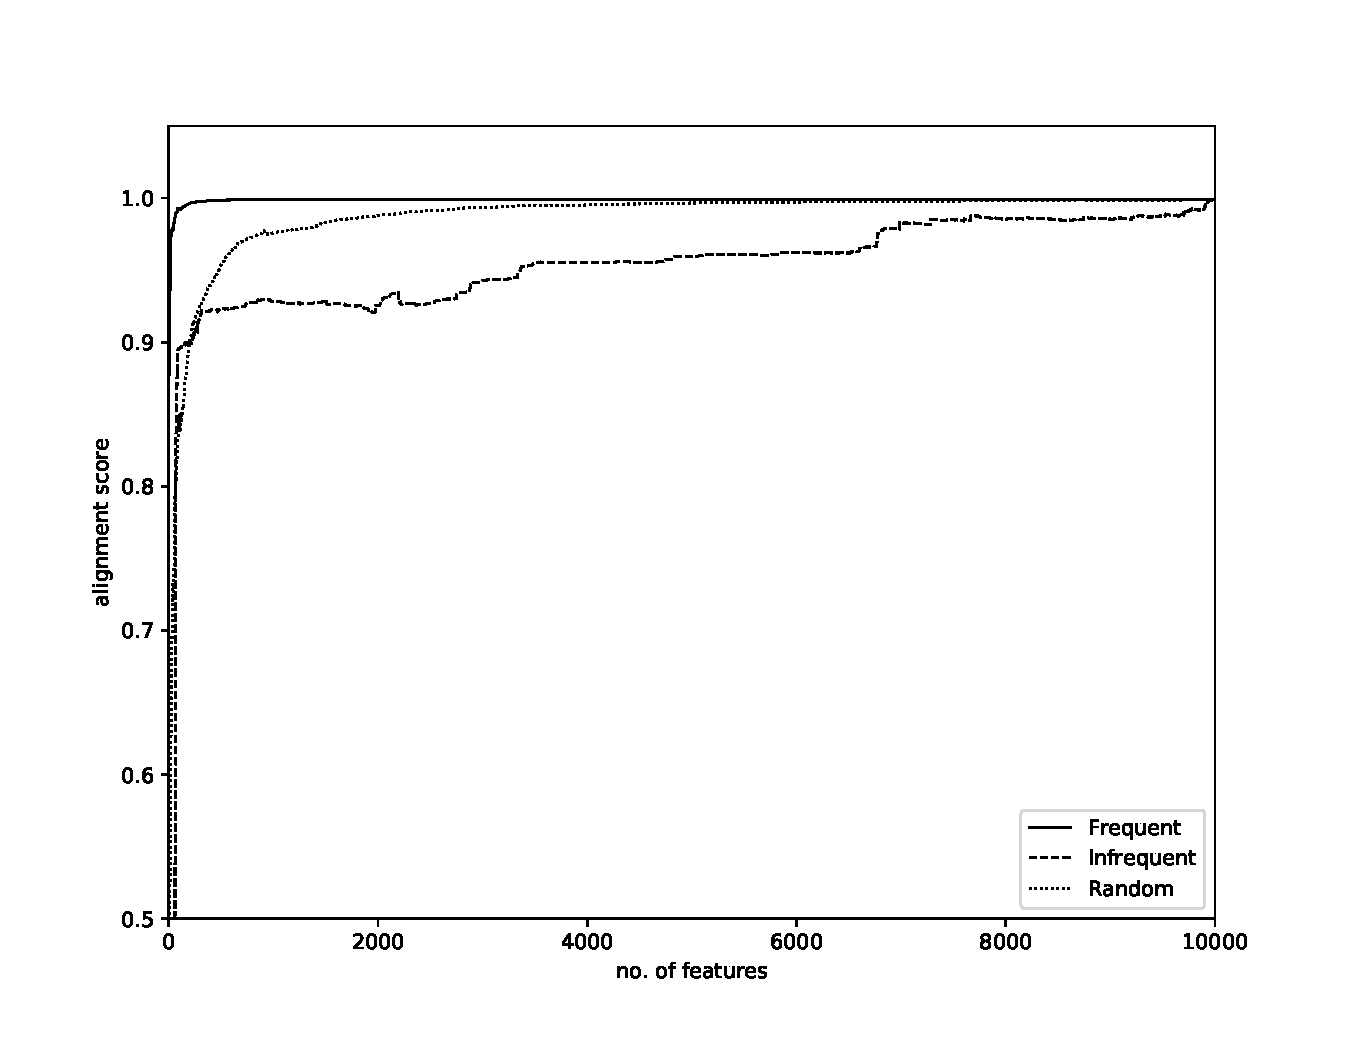
\includegraphics[height = 6.25cm]{../plots/Alignment_scores.pdf}}
	\subfloat[Lohdi et al.'s]{\raisebox{0.57cm}%
		{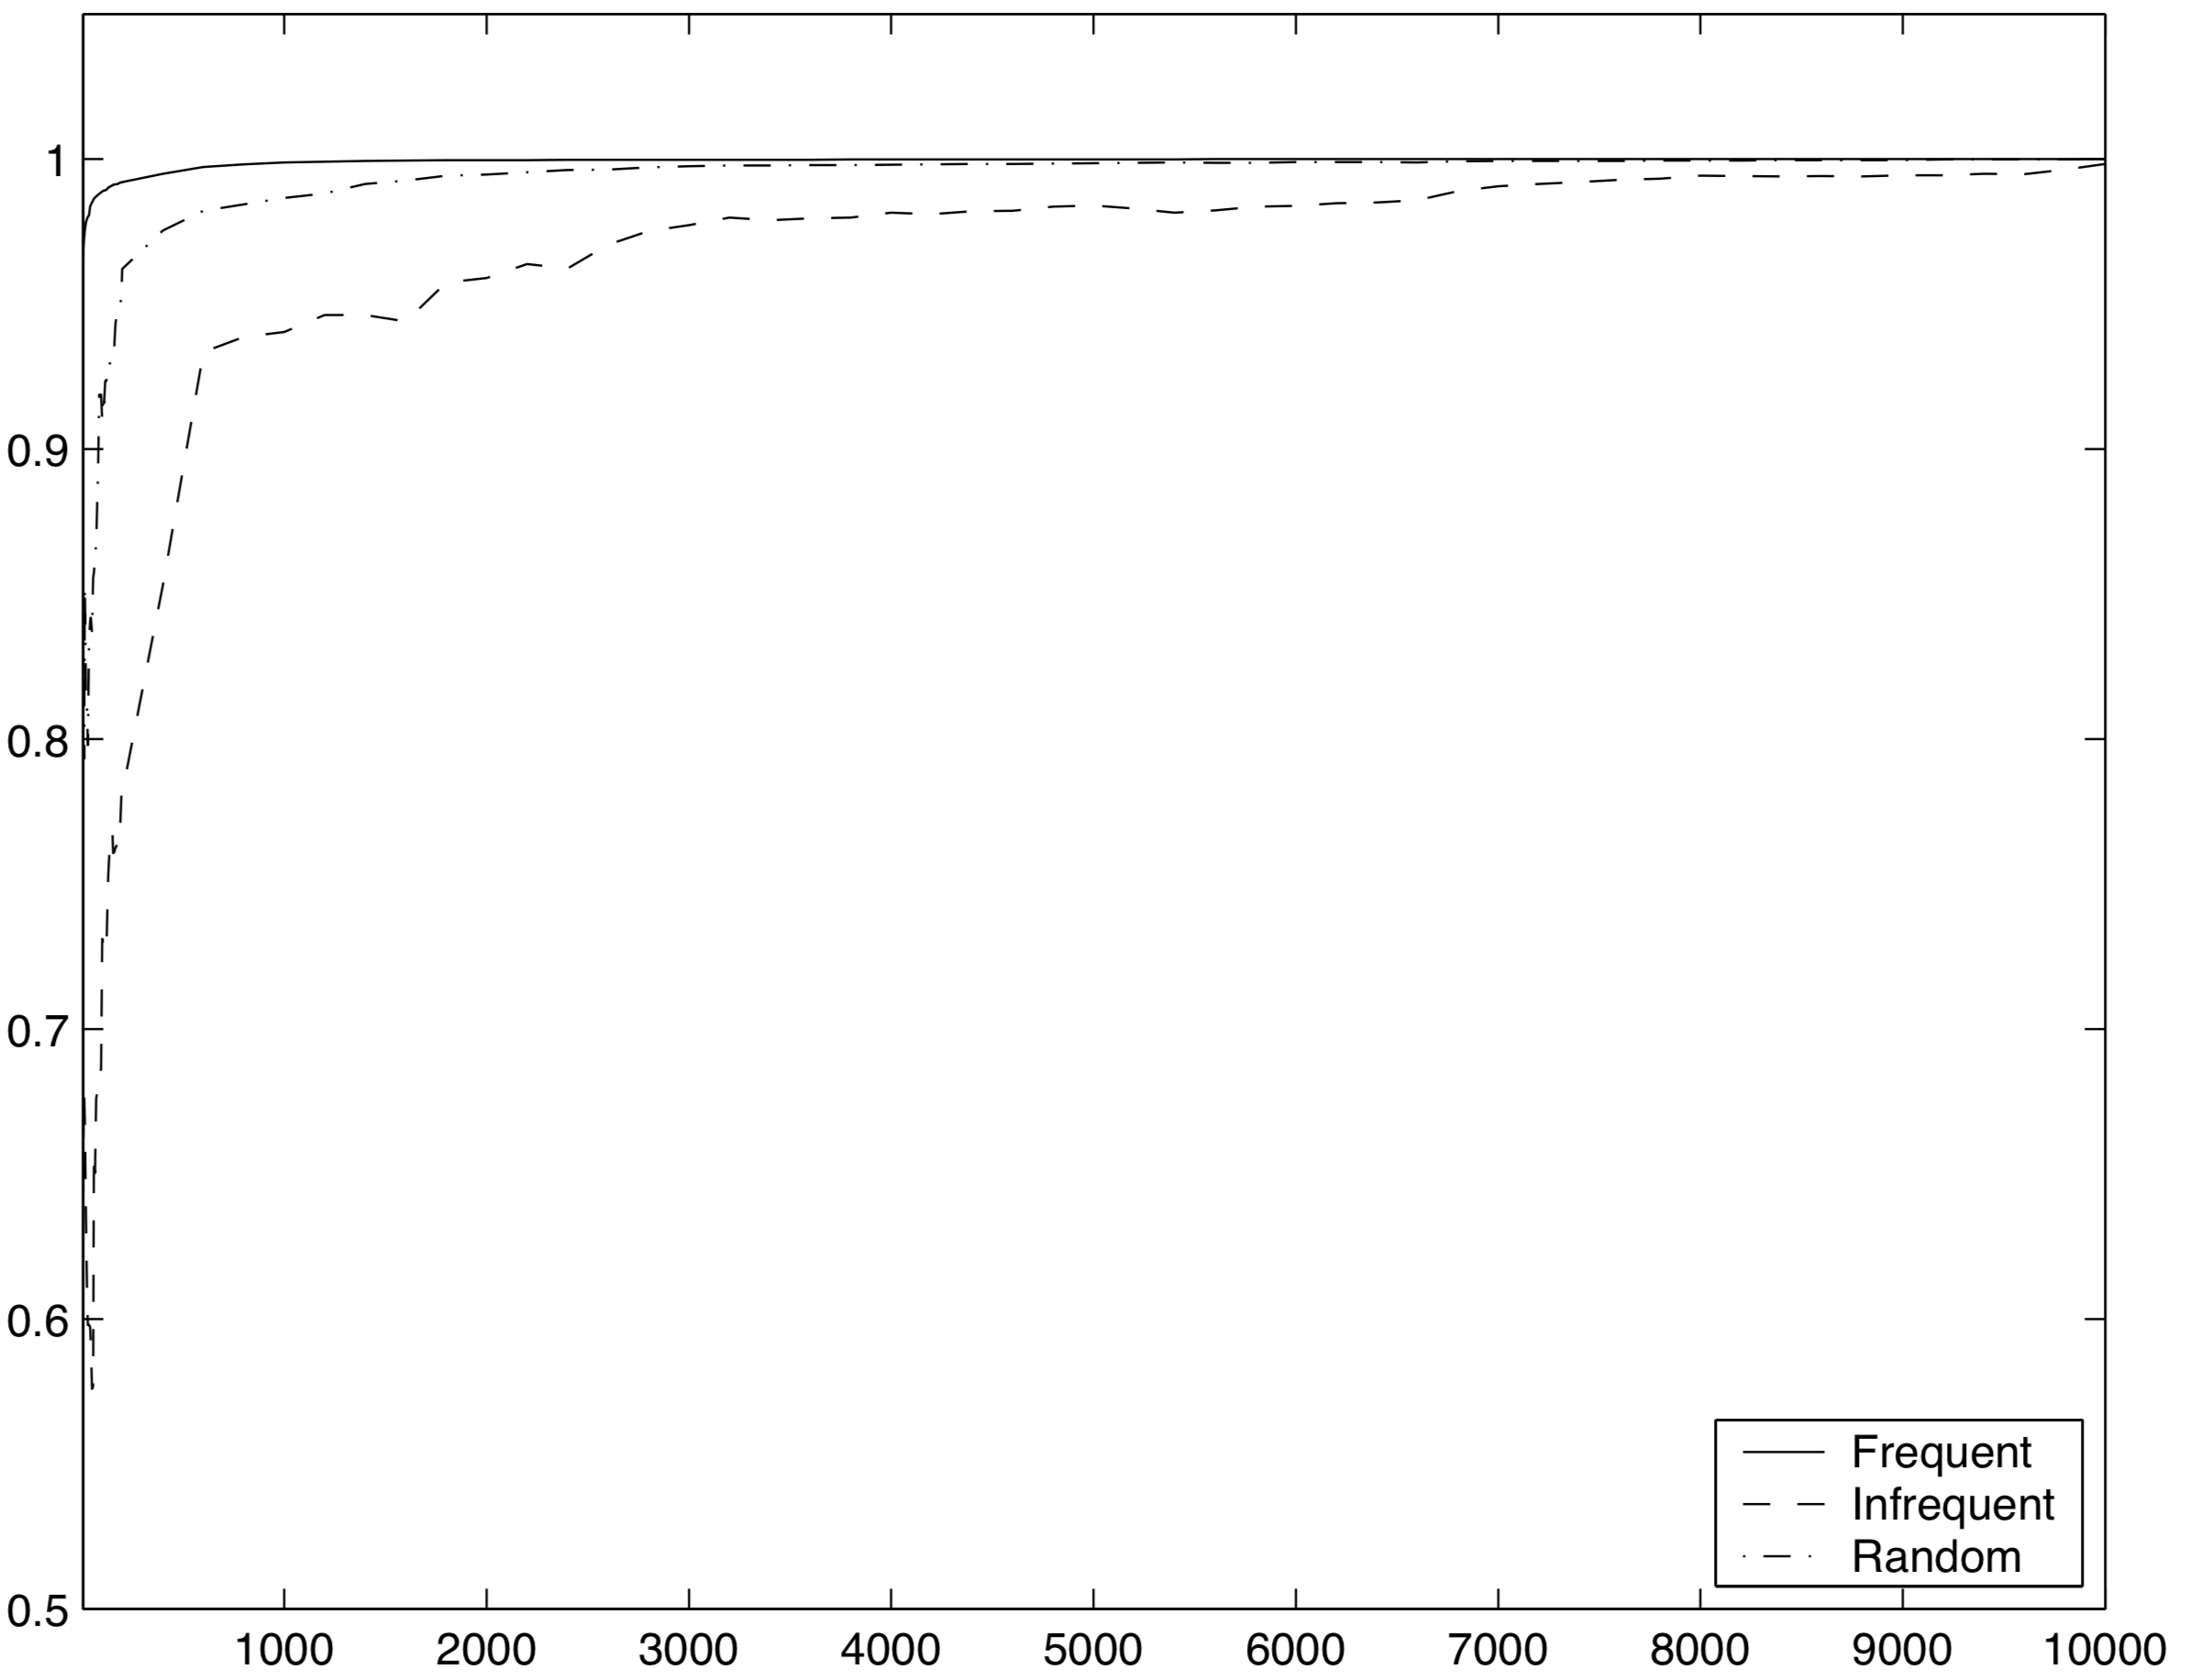
\includegraphics[height = 5cm]{../plots/Lodhi_alignment_score.png}}}%
	\caption{Alignment scores for varying the number of vectors $ x $ in the subset $ \tilde{S} $. Lohdi et al.'s figure is shown for comparison.\label{fig:alignment}}
\end{figure}

\begin{table}
	\centering
	\begin{tabular}{| c | c | c | }\hline
		aSSK & $ x $ = 1000 & $ x $ = 3000   \\ \hline
		acq & 0.96 (0.88)& 0.97 (0.85)\\ \hline
		earn & 0.98 (0.97) & 0.98  (0.97) \\ \hline
		ship & 0.43 (0.10) & 0.63  (0.53) \\ \hline
		corn & 0.84 (0.15) & 0.89 (0.65) \\ \hline
	\end{tabular} 
	\caption{F1 performance of the approximative SSK using 1000 and 3000 vectors in $ \tilde{S} $. $ n = 5 $ and $ \lambda = 0.5 $. Lodhi's results in parenthesis for comparison.\label{tab:alignment}}
\end{table}


\begin{table}
	\centering	
	\begin{tabular}{| c | c | c | c | c | c | c | c |}\hline
		& WK & NGK & NGK  & NGK  & aSSK & aSSK& aSSK \\ 
		&  & $n = 3$& $ n = 4 $ & $ n = 5 $ & $ n = 3 $& $ n = 4 $ & $ n = 5 $ \\ \hline
		earn & 0.98 & 0.98 &  0.98&  0.98 & 0.98 & 0.98 & 0.98 \\ \hline
		acq & 0.97 & 0.95 &  0.95 &  0.96 & 0.95 & 0.95 & 0.95 \\ \hline
		money-fx & 0.79 & 0.77 &  0.79 & 0.77 & 0.77 & 0.8 & 0.78 \\ \hline
		grain & 0.92 & 0.81 &  0.83& 0.82 & 0.84 & 0.86 & 0.8 \\ \hline
		crude & 0.87 & 0.84 &  0.85 & 0.8 & 0.82 & 0.79 & 0.73 \\ \hline
		trade & 0.8 & 0.73 &  0.77 & 0.77 & 0.72 & 0.79 & 0.77 \\ \hline
		interest & 0.8 & 0.72 &  0.73 & 0.75 & 0.79 & 0.8 & 0.77 \\ \hline
		ship & 0.78 & 0.66 &  0.55 & 0.47 & 0.69 & 0.5 & 0.34 \\ \hline
		wheat & 0.79 & 0.86 &  0.84 & 0.8 & 0.8 & 0.8 & 0.76 \\ \hline
		corn & 0.86 & 0.73 &  0.85 & 0.65 & 0.78 & 0.72 & 0.6 \\ \hline	
	\end{tabular}
\caption{The ten best performing classes from \cite{lodhi} shown with our $ F_1 $ results for WK, NGK and  aSSK using the entire Reuters dataset. For aSSK; $ \lambda = 0.5 $\label{tab:full_data} }
\end{table}


\subsection{Eriks kommentarer}
\begin{itemize}
	\item We can clearly see that NGK performs well for small N, but considerably worse for larger N (see appendix)
	
	\item Like it's algorithmic cousin the NGK, it performs well for relative small k, but less well for larger k (again, see appendix for all data)
	
	\item  Varying $ \lambda $ shows that SSK is not that sensitive to values of $ \lambda $. Generally we can see that unless you choose more extreme values, the SSK performs well.
	
	\item Lodhi's results in parenthesis. This allows us to verify our implementation of the approximation kernel, but is not used for extensive results analysis.
\end{itemize}

	
	\section{Discussion}
	%TODO Consequences from test runs
We can clearly see the same pattern between our data and that of Lodhi et al, that for higher $ n $ we have a clear drop off in performance. We had to limit our computations because of time limitations, but the general trend is there. Performance quickly drops of for $ n > 6 $ for almost all classes. This was consistent across all configurations of the algorithm and the approximated version. Interestingly, the results for SSK isn't super promising, we usually achieve tangential performance with either NGK and WK. This becomes painfully clear when we run the full dataset, where WK outperformed NGK and SSK on most categories at a fraction of the computation time, and that is with our approximation kernel exported to C++ and WK running completely in Python. As Lodhi summarized the findings in his report, that for small text strings and small $ n $ will the SSK perform well, but quickly losses ground. This can be very logical, since when we get more data noise to signal ratio for words goes down and we can rely more on the words rather than some sequence of characters. More documents also makes the $ tfidf $ transform better, since we get more data on which words contains information and which words are too frequent to offer distinguishing features. At the same time will stuff like n-grams and the SSK hit more noisy information since more and longer text string are bound to hit more possible combinations. Another reason for why WK works well compared to SSK might be because of the nature of the dataset. Reuters journalists are proofread and held to a higher linguistic standard than say a chat log from some messenger program. The relative lower amount of spelling errors and stylistic stringency should have a positive effect on WK's performance relative SSK. Important to note when comparing our results to \cite{lodhi2002text} is that we use a slightly smaller subset of Reuters than them. How they handled their data is not always clearly stated, so some assumptions have been made. In some cases this might provide a higher $ F_1 $ score than \cite{lodhi2002text}.
\\
As with the report from Lodhi et al, we find that SSK is not particularly sensitive to values on the decay parameter $ \lambda $, and as long as one avoids values close to one or zero the performance is generally very similar between classes. Reuters, being a unbalanced dataset creates some issues for the SVM. The disparity between classes are big, sometimes thousands to one. We've tried to solve this problem with a variety of technique, but mostly trying to balance the data so that the SVM can find decision boundary that generalizes well. What we've found though is that we didn't manage to find appropriate parameters for larger $ n $. Both NGK and SSK suffered at higher values of $ n $ and we could not replicate the performance mentioned by Lodhi et al. with many classes performing zero precision and recall. Time restrictions made tuning the parameters for the SVM to achieve acceptable results impossible for $ n \in [10,12,14] $. 
\\
%TODO Similarity to fastText and CNN and differences
Looking at the present state of natural language processing we find that currently quite a lot of hype surrounds algorithms like Convolutional Neural Networks (CNN) and \textit{fastText}. They work very differently, both from each other and SSK, but both perform very well. Use a deep network to classify text. Neural networks can be notoriously slow to train for large datasets, but generally performs very well across multiple classification and regression problems. \textit{fastText} on the other hand i very fast, capable of training and classifying large datasets in seconds SOURCE. It uses language specific precomputed vectors to classify text, but has been shown to perform similarly to CNNs on some datasets. The main benefit is the drastically quicker computation time.
\\
We looked into a method of speeding up the computations further without losing to much accuracy. Our experiments on the same four category subset of Reuters as used by Lodhi et al showed that we can achieve some reduction in time.

	
	\bibliographystyle{plain}
	\bibliography{citations.bib}
	
	%\section*{Appendix}
	%
\begin{tabular}{l r}
\begin{tabular}{| c | c | c | c | c | c | }
	\hline SSK & k&$ \lambda  $& Precision & Recall & F1   \\ \hline	
	
	&& 0.01 & 0.96 & 0.92 & 0.94  (0.873)   \\ 
	&& 0.05 & 1 & 0.92 & 0.96 (0.882)   \\ 
	acq &5& 0.1 & 1& 1 &  1 (0.871)  \\
	&& 0.5 & 0.89 & 1 & 0.94 (0.867)   \\ 
	&& 0.7 & 0.93 & 0.96 & 0.94 (0.805)    \\ 
	&& 0.9 & 0.64 & 0.96 & 0.77   (0.735)  \\ \hline
	
	
	&& 0.01 & 0.95 & 0.95 &  0.95  (0.946)  \\	
&	& 0.05 & 1 & 0.98 &  0.99  (0.946)  \\ 
	earn&5 & 0.1 & 0.98 & 1 &  0.99  (0.944)  \\ 
	&& 0.5 & 1 & 0.90 &  0.95  (0.936)  \\ 
	&& 0.7 & 1 & 0.90 &  0.95  (0.928)  \\
	&& 0.9 & 0.95 & 0.88 &  0.91  (0.914)  \\\hline
	
	
	
	&& 0.01 & 1 & 0.80 & 0.89  (0.845)   \\ 
	&& 0.05 & 1 & 0.87 & 0.93  (0.834)   \\ 
	corn&0.5 & 0.1 & 1 & 0.87 & 0.93  (0.827)   \\ 
	&& 0.5 & 0.94 & 1 &  0.97 (0.779)  \\ 
	&& 0.7 & 1 & 0.80 & 0.89   (0.628)  \\ 
	&& 0.9 & 0.64 & 0.60 & 0.62  (0.348)   \\ \hline
	
	
	&& 0.01 & 1 & 0.70 &  0.82  (0.937)  \\
	&& 0.05 & 0.90 & 0.75 &  0.82   (0.945) \\ 
	crude&5 & 0.1 & 1 & 0.91 & 0.95 (0.947)    \\ 
	&& 0.5 & 1 & 0.70 &  0.82 (0.936)   \\ 
	&& 0.7 & 0.90 & 0.90 &  0.90  (0.893)  \\
	&& 0.9 & 0.39 & 1 &  0.56  (0.758)  \\\hline
	
	
\end{tabular} &

\begin{tabular}{| c | c | c | c | c | }
	\hline NGK & k & Precision & Recall & F1   \\ \hline
	
	& 3 & 0.96 & 0.88 & 0.92 (0.791)    \\ 
	& 4 & 0.90 & 0.89 &  0.89 (0.873)   \\
	acq	& 5 & 0.97 & 0.86 & 0.92  (0.882)   \\ 
	& 6 & 0.99 & 0.82 & 0.89  (0.880)   \\
	& 7 & 0.98 & 0.79 & 0.87  (0.870)   \\
	& 8 & 1 & 0.67 & 0.80  (0.857)   \\
	\hline
	
	
	
	& 3 & 0.97 & 0.93 &  0.95 (0.919)   \\ 
	& 4 & 0.99 & 0.93 &  0.96 (0.943)   \\ 
	earn & 5 & 0.99 & 0.89 &  0.93  (0.944)  \\ 
	& 6 & 0.99 & 0.89 &  0.93  (0.943)  \\ 
	& 7 & 0.99 & 0.89 &  0.93  (0.940)  \\ 
	& 8 & 0.99 & 0.89 &  0.93  (0.940)  \\ \hline
	
	
	
	& 3 & 1 & 0.87 & 0.93  (0.797)   \\ 
	& 4 & 1 & 0.64 & 0.78  (0.841)   \\ 
	corn	& 5 & 1 & 0.44 &  0.61 (0.847)   \\ 
	& 6 & 1 & 0.42 & 0.59  (0.815)   \\ 
	& 7 & 1 & 0.24 & 0.38  (0.767)  \\ 
	& 8 & 1 & 0.28& 0.42  (0.706)   \\ \hline
	
	
	& 3 & 0.90 & 0.90 &  0.90  (0.907)  \\ 
	& 4 & 0.92 & 0.86 & 0.89  (0.935)   \\ 
	crude & 5 & 1 & 0.73 &  0.84 (0.937)   \\ 
	& 6 & 1 & 0.66 &  0.79 (0.908)   \\
	& 7 & 1 & 0.60 &  0.72 (0.904)   \\
	& 8 & 1 & 0.28 &  0.44  (0.869)  \\ \hline
	
	
	
\end{tabular} \vspace{10pt} \\ 


\begin{tabular}{| c | c | c | c | c | c | }
	\hline SSK&$ \lambda $& k & Precision & Recall & F1   \\ \hline


			
	
	&& 3 & 0.93 & 0.96 & 0.94 (0.785)    \\ 
	&& 4 & 0.93 & 0.96 &  0.94  (0.822)  \\
	acq	&0.5& 5 & 0.97 & 0.93 & 0.95  (0.867)   \\ 
	&& 6 & 0.98 & 0.93 & 0.95 (0.876)    \\
	&& 7 & 0.98 & 0.89 & 0.93 (0.864)    \\
	&& 8 & 0.99 & 0.80 & 0.93  (0.852)   \\\hline
	
	
	
	&& 3 & 0.99 & 0.93 & 0.96  (0.925)   \\ 
&& 4 & 0.99 & 0.95 &  0.97  (0.932) \\
earn&0.5	& 5 & 0.99 & 0.96 & 0.97   (0.936)  \\ 
&& 6 & 0.99 & 0.93 & 0.97  (0.936)   \\
&& 7 & 0.99 & 0.91 & 0.96 (0.940)    \\
&& 8 & 0.99 & 0.86 & 0.95  (0.934)   \\\hline

	
	
	
	&& 3 & 0.97 & 0.87 & 0.91  (0.665)   \\ 
	&& 4 & 0.98 & 0.64 & 0.88  (0.783)   \\ 
	corn&0.5	& 5 & 0.98 & 0.44 &  0.83  (0.779)  \\ 
	&& 6 & 0.98 & 0.42 & 0.78   (0.749)  \\ 
	&& 7 & 0.98 & 0.24 & 0.74  (0.643)  \\ 
	&& 8 & 1 & 0.28& 0.59  (0.569)   \\ \hline
	
	
	&& 3 & 0.97 & 0.86 &  0.88  (0.881)  \\ 
	&& 4 & 0.98 & 0.80 & 0.91  (0.905)   \\ 
	crude &0.5& 5 & 0.98 & 0.73 &  0.88 (0.936)   \\ 
	&& 6 & 0.98 & 0.66 &  0.82  (0.901)  \\
	&& 7 & 0.98 & 0.60 &  0.73 (0.872)  \\
	&& 8 & 1 & 0.43 &  0.67   (0.828) \\ \hline 
	
	
	
\end{tabular} &

\end{tabular} % This is the end tabular





\end{document}